\documentclass{article}

\usepackage{graphicx}
\usepackage{tikz}
\usepackage{tikzsymbols}
\usetikzlibrary{calc,patterns,shapes.geometric}
\pagestyle{empty}
\usepackage[margin=0pt]{geometry}
\geometry{papersize={14in,12in}}

\def\centerarc[#1](#2)(#3:#4:#5){\draw[#1] ($(#2)+({#5*cos(#3)},{#5*sin(#3)})$) arc (#3:#4:#5);}

\begin{document}
	\begin{figure}
		\centering
		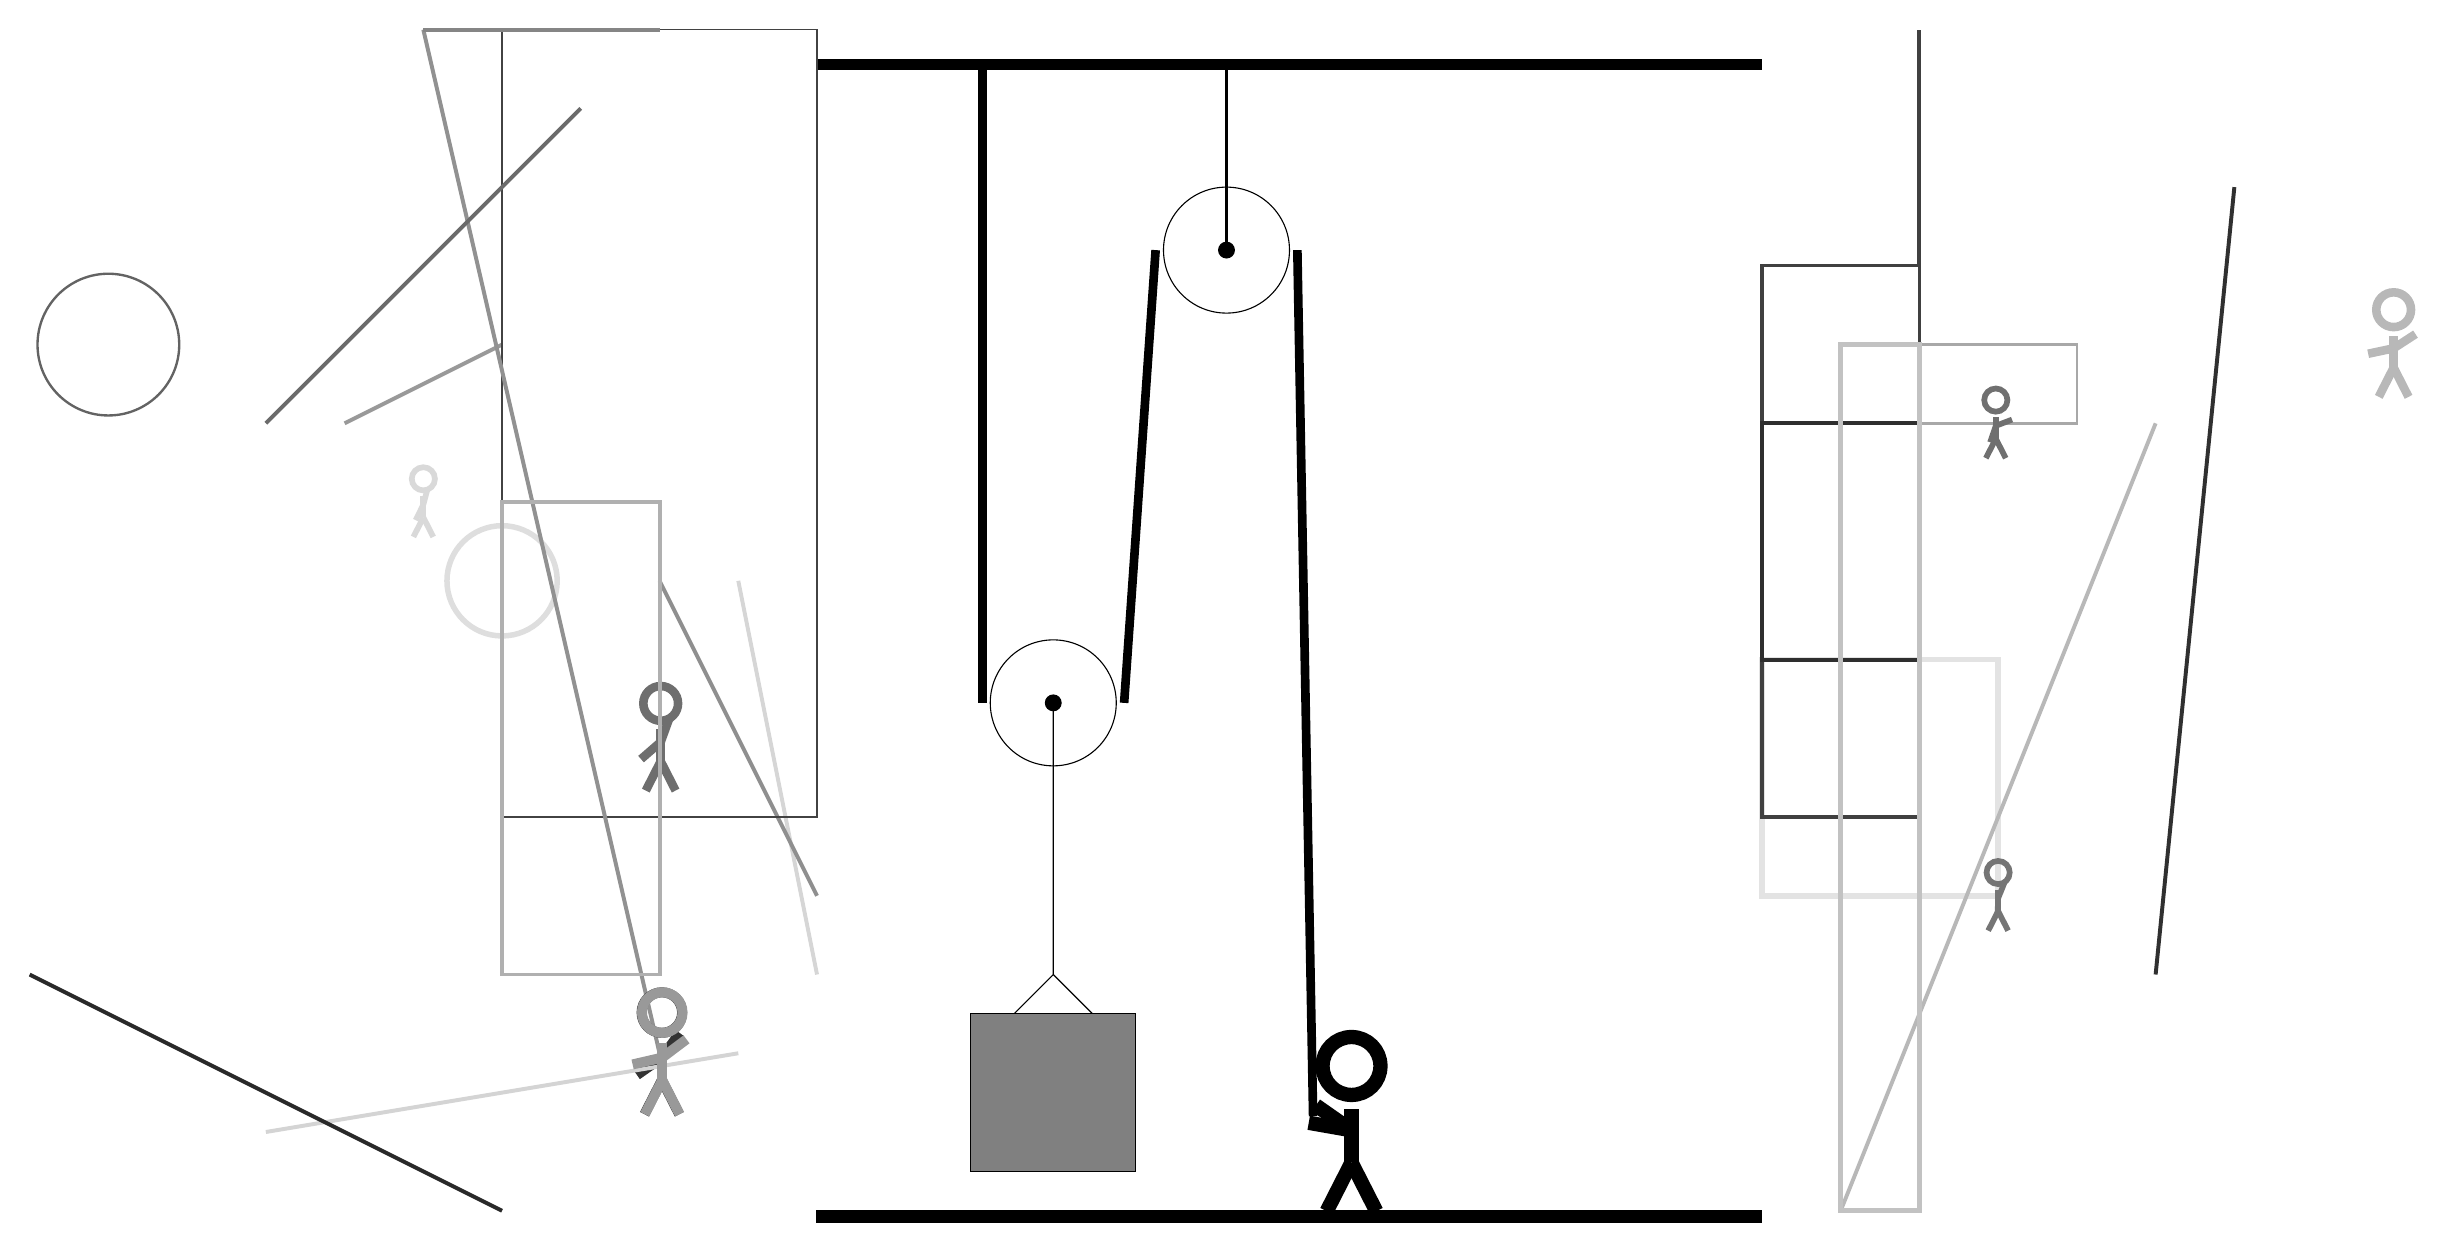
\begin{tikzpicture}
			%%%%% START %%%%%
			
			\draw[fill=black] (-2, 11.5) rectangle (10, 11.625);
			
			\draw (3.2, 9.2) circle (0.8);
			\draw[fill=black] (3.2, 9.2) circle (0.1);
			\draw[thick] (3.2, 9.2) -- (3.2, 11.5);
			
			\draw (1, 3.45) circle (0.8);
			\draw[fill=black] (1, 3.45) circle (0.1);
			
			\draw (1, 3.45) -- (1, 0.0) -- (0.5, -0.5);
			\draw (1, 0.0) -- (1.5, -0.5);
			\draw[fill=black!50] (-0.05, -0.5) rectangle (2.05, -2.5);
			
			\draw[line width=0.3mm, color=black!34] (12, 7) rectangle (14, 8);
			
			\draw[line width=0.5mm, color=black!16](-3, 5) -- (-2, 0);
			\draw [line width=0.7mm, color=black!13](-6, 5) circle (0.7);
			\node[line width=0.4mm, color=black!56] at (13, 7) {\Strichmaxerl[4][71][21]};
			\node[line width=0.7mm, color=black!57] at (-4, 3) {\Strichmaxerl[6][41][70]};
			
			\node[line width=0.2mm, color=black!28] at (18, 8) {\Strichmaxerl[6][12][33]};
			
			\draw[line width=0.5mm, color=black!44](-2, 1) -- (-4, 5);
			\draw[line width=0.7mm, color=black!11] (10, 1) rectangle (13, 4);
			\draw[line width=0.5mm, color=black!40](-6, 8) -- (-8, 7);
			\draw[line width=0.2mm, color=black!74] (-2, 2) rectangle (-6, 12);
			
			\draw [line width=0.3mm, color=black!61](-11, 8) circle (0.9);
			\draw[line width=0.4mm, color=black!75] (12, 2) rectangle (10, 9);
			\draw[line width=0.5mm, color=black!82] (12, 4) rectangle (10, 7);
			\draw[line width=0.5mm, color=black!43](-4, -1) -- (-7, 12);
			\draw[line width=0.5mm, color=black!28](11, -3) -- (15, 7);
			\node[line width=0.5mm, color=black!54] at (13, 1) {\Strichmaxerl[4][88][68]};
			
			\node[line width=0.2mm, color=black!80] at (-4, -1) {\Strichmaxerl[7][35][54]};
			\draw[line width=0.5mm, color=black!75](12, 9) -- (12, 12);
			\draw[line width=0.6mm, color=black!24] (12, 8) rectangle (11, -3);
			
			\draw[line width=0.5mm, color=black!17](-3, -1) -- (-9, -2);
			\draw[line width=0.5mm, color=black!58](-5, 11) -- (-9, 7);
			
			\draw[line width=0.5mm, color=black!48](-4, 12) -- (-7, 12);
			\draw[line width=0.5mm, color=black!81](15, 0) -- (16, 10);
			\node[line width=0.7mm, color=black!15] at (-7, 6) {\Strichmaxerl[4][64][75]};
			\node[line width=0.5mm, color=black!40] at (-4, -1) {\Strichmaxerl[7][13][37]};
			
			\draw[line width=0.5mm, color=black!31] (-4, 0) rectangle (-6, 6);
			\draw[line width=0.5mm, color=black!84](-6, -3) -- (-12, 0);
			
			\draw[line width=1.1mm] (0.1, 11.5) -- (0.1, 3.45);
			\centerarc[line width=1.1mm](1, 3.45)(180:360:0.9);
			\draw[line width=1.1mm](1.9, 3.45) -- (2.3, 9.2);
			\centerarc[line width=1.1mm](3.2, 9.2)(0:180:0.9);
			\draw[line width=1.1mm](4.1, 9.2) -- (4.3, -1.8);
			
			\node at (4.7, -1.9) {\Strichmaxerl[10][-35][170]};
			
			\draw[fill=black] (-2, -3) rectangle (10, -3.15);
			
			%%%%% END %%%%%
		\end{tikzpicture}
	\end{figure}	
\end{document}